\section{National products and results}\label{sec:results}
\subsection{Native gases and GWP aggregates}
Reference S\_TAN produces \SI{\PakRefARfive}{\mega\tonne} CO$_2$-equivalent in FY2023--24 and \SI{\PakLatestARfive}{\mega\tonne} in FY2024--25 on AR5 GWP-100. Reference native masses are \SI{\PakRefCOtwo}{\mega\tonne} CO$_2$, \SI{\PakRefCHfour}{\giga\gram} CH$_4$ and \SI{\PakRefNtwoO}{\giga\gram} N$_2$O. AR6 aggregates are \SI{\PakRefARsix}{\mega\tonne} and \SI{\PakLatestARsix}{\mega\tonne}, respectively. The supported scope remains non-LULUCF and excludes explicit missing categories.

\begin{table}[htbp]\centering\small
\begin{tabular}{@{}lrr@{}}\toprule
Native core species (Gg) & FY2023--24 & FY2024--25\\\midrule
PM$_{2.5}$ & \PakRefPMfine & \PakLatestPMfine\\
BC & \PakRefBC & \PakLatestBC\\
NO$_x$ (NO$_2$-equivalent) & \PakRefNOx & \PakLatestNOx\\
SO$_2$ & \PakRefSOtwo & \PakLatestSOtwo\\
CO & \PakRefCO & \PakLatestCO\\
NMVOC & \PakRefNMVOC & \PakLatestNMVOC\\
NH$_3$ & \PakRefNHthree & \PakLatestNHthree\\\bottomrule
\end{tabular}
\caption{Covered-source air estimates from the current release. Nested particulate species are non-additive.}\label{tab:air_current}
\end{table}

Household combustion supplies approximately two-thirds of reference covered PM$_{2.5}$; open waste and field burning are substantial additional sources. Nitrogen pathways dominate NH$_3$. NO$_x$ and SO$_2$ retain different fuel, industrial and control contributions. These are specific source comparisons, not an inverse ordering of GHG and air emissions or an exposure ranking.

\begin{figure}[htbp]\centering
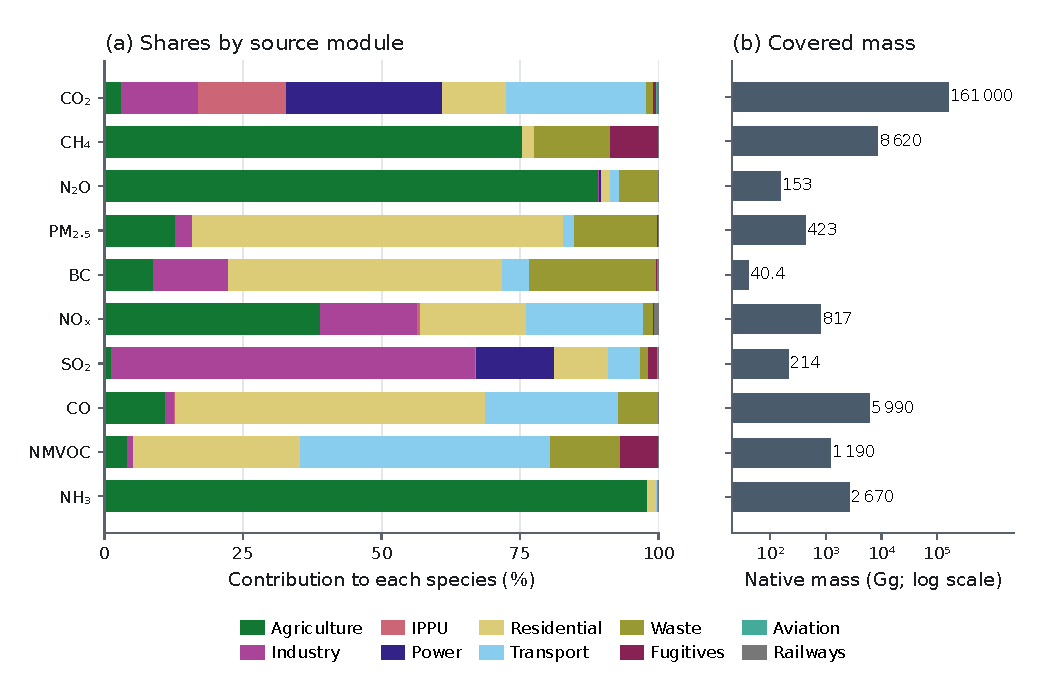
\includegraphics[width=\linewidth]{f09_integrated_composition.pdf}
\caption{Reference source contributions within each species and separate native mass. Shares and absolute quantities answer different questions; the mass axis is logarithmic. Data accompany the figure.}\label{fig:sectors}
\end{figure}

\subsection{Historical change}\label{sec:series}\label{sec:agri-basis}\label{sec:waste-series}
The common panel contains ten fiscal years, July 2015--June 2025. Between FY2015--16 and FY2024--25, covered AR5 GHG changes by \SI{\PakChangeARfive}{\percent}, PM$_{2.5}$ by \SI{\PakChangePMfine}{\percent}, NO$_x$ by \SI{\PakChangeNOx}{\percent}, SO$_2$ by \SI{\PakChangeSOtwo}{\percent} and NH$_3$ by \SI{\PakChangeNHthree}{\percent}. The provisional FY2025--26 source extension is excluded from these endpoints.

Station consumption, sales, crop and nutrient observations supply measured activity changes where available. Census-anchored herd reconstruction, household interpolation/extrapolation and fixed fate parameters supply modelled changes. Coal consumer allocations and edition revisions can cause important industrial changes; a shift in booked kiln fuel is not evidence of a regulatory change in district emissions. Waste history is advanced consistently. Older 1990 calendar diagnostics remain separate and are not spliced onto the common core as uniform fiscal observations.

\begin{figure}[htbp]\centering
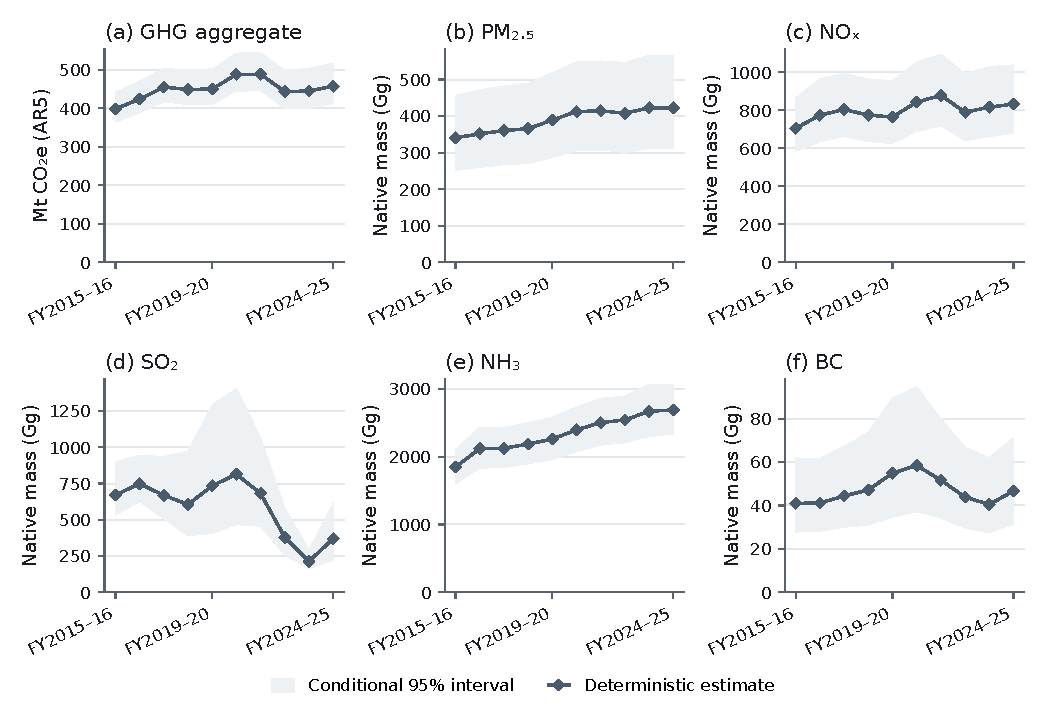
\includegraphics[width=\linewidth]{f10_integrated_trends.pdf}
\caption{Fiscal trends and conditional persistent-parameter intervals. Structural alternatives and missing categories remain outside these intervals. The common core ends in June 2025.}\label{fig:series}
\end{figure}

\subsection{Monthly allocation}\label{sec:monthly}
Annual compatible estimates are allocated through source/process profiles,
\begin{equation}E_{s,p,m}=E_{s,p,t}w_{s,p,m},\qquad\sum_{m\in t}w_{s,p,m}=1.\label{eq:monthly}\end{equation}
Production or sales can be a proxy for emission timing. Fertiliser offtake is supply timing rather than observed application; manure-stage and residue-decomposition release dates are unobserved. Road evaporation and wear do not inherit an observed exhaust fuel profile without evidence. Waste burning, annual flare quantities and unsupported releases retain declared fallbacks. The admitted station subset's aggregate fleet timing is labelled a proxy.

The repaired PBS extraction preserves centred labels, continuation/province rows, source units and worksheet identity. Actual exported province/month values and compatible monthly/annual controls determine admission. Surviving source anomalies are flagged, and national monthly classification requires producing-area completeness; missing observations are not converted to zero. Temporal evidence shares are calculated separately by pollutant.

\subsection{Administrative and grid products}\label{sec:cube}
Source-matched annual weights produce ADM1, ADM2 and 0.05$^\circ$ cell masses under each configuration. Facilities respect commissioning/closure; selected oil/diesel stations use their admitted subset frame, and kiln types retain the supported frame plus an unlocated remainder. Rail geometry excluded from the compatible primary package retains supported administrative mass and explicit fine-scale unallocated mass. Fixed proxies and reference-year patterns retain their evidence class.

\begin{figure}[htbp]\centering
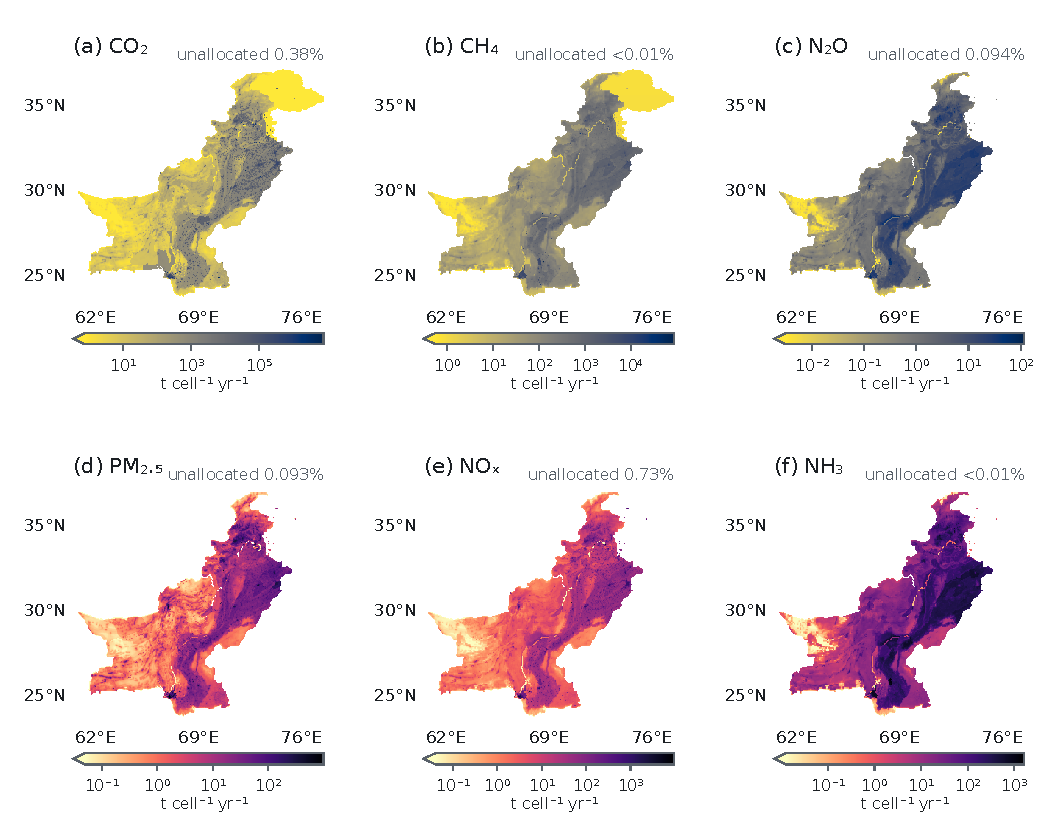
\includegraphics[width=\linewidth]{f11_integrated_maps.pdf}
\caption{Reference native gas and pollutant mass per cell, with separate logarithmic scales. Geographic weights can describe release location, activity origin or accounting; fixed allocation is not observed local change. Unallocated mass is published separately.}\label{fig:maps}
\end{figure}

For each species/configuration/period, annual--monthly and placed--unallocated closure is tested at compatible boundaries. Cell mass is distinct from flux density. Area, country fraction where relevant and duration are required for conversion; vertical injection and detailed chemical speciation remain additional atmospheric-model requirements.
